\newpage
\datos{color}{}{}
\section*{Propuesta técnica de búsqueda local}
\addcontentsline{toc}{section}{Propuesta técnica de búsqueda local}

\subsection*{Algoritmo elegido}
\addcontentsline{toc}{subsection}{Algoritmo elegido}

Se ha seleccionado el algoritmo de Temple Simulado (\textit{Simulated Annealing}, SA) 
dado que el espacio de búsqueda es continuo y existen restricciones geométricas 
y cinemáticas no triviales. Las variables incluyen posiciones en $\mathbb{R}^3$, orientaciones en forma de cuaterniones unitarios
y factores de velocidad acotados, lo que dificulta la definición de vecindarios discretos o estructuras
de memoria como las empleadas en Búsqueda Tabú. En cambio, El Temple Simulado permite explorar este espacio
continuo mediante perturbaciones suaves y controladas.

\subsection*{Diseño del algoritmo}
\addcontentsline{toc}{subsection}{Diseño del algoritmo}

\subsubsection*{Representación de las soluciones}
Cada solución candidata se representa como un vector continuo:
\[
\mathbf{x} =
(\mathbf{p}_A,\mathbf{p}_B,
\mathbf{q}_A,\mathbf{q}_B,
s_A,s_B,s_{rail})
\in \mathbb{R}^{17},
\]

donde $\mathbf{p}_A, \mathbf{p}_B \in \mathbb{R}^3$ son las posiciones objetivo de cada robot,
$\mathbf{q}_A, \mathbf{q}_B \in S^3$ son cuaterniones unitarios que representan orientaciones de cada efector y
$s_A, s_B, s_{rail} \in (0,1]$ son los factores de velocidad de cada robot y del motor lineal de desplazamiento.

\subsubsection*{Operadores de vecindad}
El operador de vecindad genera una solución cercana mediante una perturbación gaussiana,
$\mathbf{x}' = \mathbf{x} + \mathcal{N}(0,\sigma^2)$, pero adaptada a la naturaleza de cada 
tipo de variable:

\begin{itemize}
    \item \textbf{Posiciones}: 
    $\mathbf{p}_r' = \mathbf{p}_r + \mathcal{N}(0,\sigma_p^2),$
    seguidas de una proyección al espacio de trabajo mediante truncamiento si alguna coordenada sale de los límites. 
    Esta operación asegura que $\mathbf{p}_r' \in \mathcal{W}_r$ tras la mutación:
    $p_{r,i}' \leftarrow 
    \min\big(p_{i,\max},\, \max(p_{i,\min},\, p_{r,i}')\big),
    \qquad i \in \{x,y,z\}.
    $
    
    \item \textbf{Orientaciones}:
    $\mathbf{q}_r' = \mathbf{q}_r + \mathcal{N}(0,\sigma_q^2),$
    donde el cuaternión resultante se vuelve a normalizar para garantizar que es unitario:
    $\mathbf{q}_r' \leftarrow \frac{\mathbf{q}_r'}{\|\mathbf{q}_r'\|}$.

    \item \textbf{Velocidades}:
    $
    s_r' = s_r + \mathcal{N}(0,\sigma_s^2),$ aplicando truncamiento para mantener la factibilidad física.
    $s_r' \leftarrow \min(1,\max(0,s_r'))$.
\end{itemize}

\subsubsection*{Gestión de restricciones}

Los operadores de vecindad garantizan únicamente la factibilidad básica de las
variables (\textit{workspace}, cuaterniones unitarios y velocidades en $[0,1]$). El resto
de restricciones del problema se gestionan en
la fase de evaluación de la solución:
\begin{itemize}
    \item \textbf{Separación y alineación}:  
    las penalizaciones $P_{\text{sep}}$ y $P_{\text{alineación}}$ cuantifican la
    desviación respecto a la configuración de \textit{rendezvous} deseada.

    \item \textbf{Sincronización temporal}:  
    se penaliza mediante $P_{\text{sync}}$.

    \item \textbf{Factibilidad cinemática y singularidades}:  
    Para cada pose candidata se verifica la existencia de una solución de
    cinemática inversa. Si no existe, la solución se descarta o penaliza mediante $P_{\text{sing}}$.  
\end{itemize}

De este modo, el Temple Simulado explora libremente el espacio de búsqueda,
mientras que la función de evaluación guía la convergencia hacia soluciones que
cumplen las restricciones.

\subsection*{Configuración de parámetros}
\addcontentsline{toc}{subsection}{Configuración de parámetros}
Se propone comenzar con una temperatura de $T_0 = 1$, un factor de enfriamiento
$\alpha = 0.95$, un máximo de $L = 50$ movimientos o generación de vecinos por temperatura,
un máximo de $K = 200$ temperaturas y una desviación del operador de vecindad de $\sigma = 0.1$.
Esta configuración permite explorar $K \cdot L = 200 \cdot 50 = 10.000$ soluciones diferentes.

\begin{comment}
    \begin{itemize}
    \item Temperatura inicial: $T_0 = 1$
    \item Factor de enfriamiento: $\alpha = 0.95$
    \item Iteraciones (movimientos) por temperatura: $L = 50$
    \item Número máximo de iteraciones (temperaturas): $K = 200$
    \item Desviación del operador de vecindad: $\sigma = 0.1$
\end{itemize}
\end{comment}

\subsection*{Diseño experimental}
\addcontentsline{toc}{subsection}{Diseño experimental}
El plan de experimentación constará de 30 ejecuciones independientes 
cada una con una semilla aleatoria distinta, de tal forma que se garantice la validez 
estadística. \\

Las soluciones se evaluarán mediante tres métricas: calidad, tiempo de ejecución y número de evaluaciones.
La calidad registra el mejor y peor 
valor final de $T_{\max}$, la media, la desviación típica y el intervalo de confianza. El tiempo
de ejecución mide el tiempo total de \textit{CPU} y se considera con la calidad de la
solución lograda. Esta consideración se realizará a través de un diagrama de dispersión, como 
el de la Figura \ref{fig:scatterPlotPropuesta}, y 
un valor de eficiencia calculado: $E = \frac{T_{max}}{\text{tiempo}}$. Por último,
el número de evaluaciones anota la iteración en la que se alcanzó el mejor valor. \\

Además, dado que el problema incluye restricciones que pueden invalidar una solución,
se registrará también la factibilidad de cada solución. A partir de ello se calculará
el porcentaje de soluciones factibles obtenidas por el algoritmo.

\subsection*{Resultados (esquema)}
\addcontentsline{toc}{subsection}{Resultados (esquema)}
Se presentan las Tablas \ref{tab:tema2_tabla1} y \ref{tab:tema2_tabla2} y la Figura 
\ref{fig:scatterPlotPropuesta} que se pretenden obtener para evaluar los resultados 
del algoritmo.

\begin{table}[H]
\centering
\begin{tabular}{|c|c|c|c|c|c|}
\hline
Ejecución & $T_{\max}$ final & Tiempo (s) & Iteración óptima & Eficiencia & \% soluciones factibles \\
\hline
1 & -- & -- & -- & -- & --\\
2 & -- & -- & -- & -- & --\\
3 & -- & -- & -- & -- & --\\
\vdots & \vdots & \vdots & \vdots & \vdots & \vdots\\
30 & -- & -- & -- & -- & --\\
\hline
\end{tabular}
\caption{Resultados individuales de las 30 ejecuciones del algoritmo.}\label{tab:tema2_tabla1}
\end{table}

\begin{table}[H]
\centering
\begin{tabular}{|l|c|}
\hline
\textbf{Métrica} & \textbf{Valor} \\
\hline
Media de $T_{\max}$ & -- \\
Desviación típica & -- \\
Mejor valor (mínimo) & -- \\
Peor valor (máximo) & -- \\
Intervalo de confianza 95\% & -- \\
Tiempo medio de ejecución (s) & -- \\
\% soluciones factibles & -- \\
\hline
\end{tabular}
\caption{Métricas agregadas calculadas sobre las 30 ejecuciones.}\label{tab:tema2_tabla2}
\end{table}

\begin{figure}[H]
  \centering
  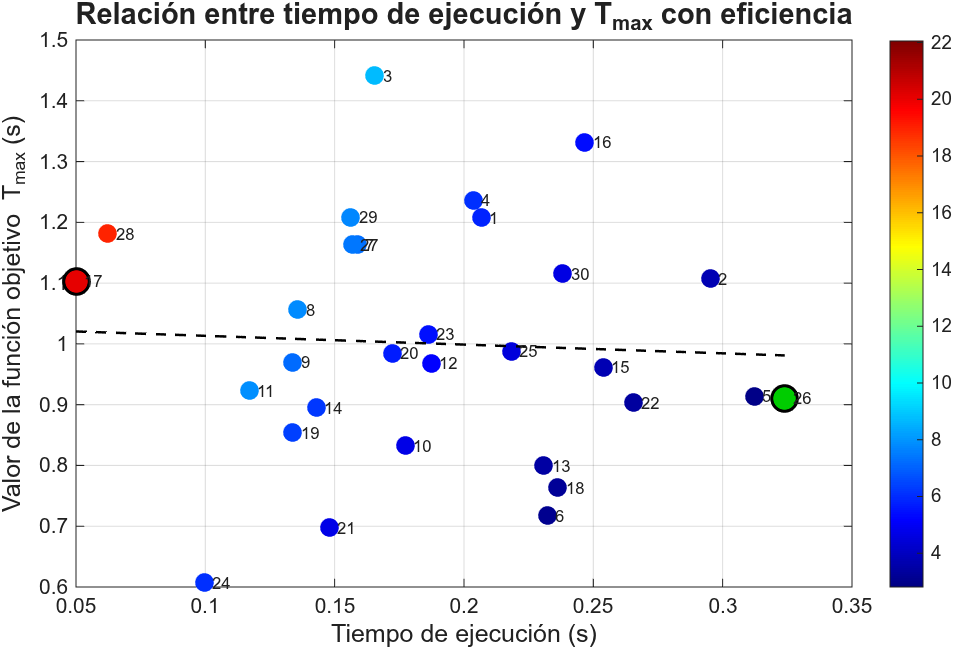
\includegraphics[scale=0.6]{Images/tema2/scatter_plot_propuesta.png}
  \caption{Diagrama de dispersión propuesto para la evaluación de la eficiencia de las soluciones. 
  Cada círculo representa una solución cuyo número adjunto corresponde con el número de ejecución, 
  el color de las soluciones se refiere a la eficiencia de las mismas, los círculos con borde negro
  representan las peor y mejor solución, en color rojo y verde, respectivamente, y la recta punteada 
  la línea de tendencia.}
  \label{fig:scatterPlotPropuesta}
\end{figure}

\subsection*{Conclusiones (expectativas)}
\addcontentsline{toc}{subsection}{Conclusiones (expectativas)}
Se espera que el Temple Simulado sea capaz de identificar configuraciones de
\textit{rendezvous} que reduzcan el valor de $T_{\max}$ y, por tanto, mejoren la
sincronización entre los dos robots. Dado que el problema combina posiciones,
orientaciones y factores de velocidad, el algoritmo debería explorar de forma
eficiente regiones del espacio de búsqueda que no serían accesibles mediante
métodos deterministas o gradientes locales. \\

Además, se busca ajustar automáticamente los factores de velocidad para compensar las
diferencias cinemáticas entre robots y el eje lineal. \\

Se considerará que el Temple Simulado constituye una estrategia válida para la
optimización del \textit{rendezvous} cooperativo si logra reducir $T_{\max}$ de
forma estable y reproducible respecto del punto de partida, si muestra 
estabilidad de los valores finales en las últimas iteraciones, es decir, convergencia,
y si el diagrama de dispersión muestra una tendencia alineada con el objetivo del problema.